\emph{This section is largely based on an article by Sean Baron, User Experience Resercher at Microsoft Game
Studios\cite{baron}.}
\emph{Cognitive Flow} is the the psychological term for being ``in the zone''. Those times when you play a game and
time flies by, without you even noticing. 
This is illustrated in Figure \ref{gamedesign:flowzone}, where the goal is
to remain inside the flow zone for the duration of the game.
\begin{figure}
    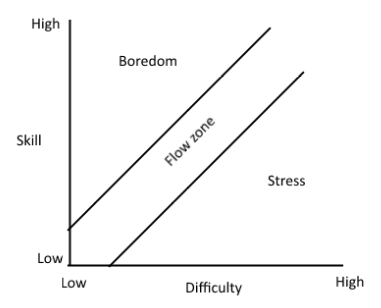
\includegraphics[scale=0.5]{figures/gamedesign/flowZone}
    \caption{Illustration of the flow zone.}
    \label{gamedesign:flowzone}
\end{figure}

To increase the chance of reaching this cognitive flow, four main states in terms of game to player interaction has to
be promoted.  These four states are 
\begin{itemize}
    \item \emph{concrete goals with manageable rules}
    \item \emph{goals that fit player capabilities}
    \item \emph{clear and timely feedback}
    \item \emph{remove distractions from player focus}
\end{itemize} While these states are fulfilled, the player will experience:

\begin{itemize}
    \item Extreme focus on task
    \item A sense of active control
    \item Merging of action and awareness
    \item Loss of self-awareness
    \item Distortion of the experience of time
    \item The experience of the task being the only necessary justification for continuing it
\end{itemize}

In other words, the player will be fully engulfed in the playing-experience of the game.

\subsection{Concrete goals with manageable rules}
This state has to do with limiting the information flow, and the amount of inputs the player has to handle at once. If
the input follows the same rules and work towards the same goal, then they are fine. If, however, they distract the
player and work against each other, the player will feel at a loss and not know what to do. For instance; The player is
receiving a quest which tells him where to go next. Whilst talking to the quest giver, the city comes under attack and
the player helps slay the monsters. Now the player has forgotten, or did not manage to read the entire prologue for the
next goal/task, and does not know where to go. The result is a feeling of not being able to accomplish the goal at
hand, leaving the player frustrated.  A way to deal with this, is by having a lot of feedback whenever goals or
part-goals are achieved. For instance, letting the player know he levelled up, or letting him know he is doing good
when making combos. This means that the game interface and game design has to help the player focus on the task at
hand. It is important, however, that no goal is neither too trivial or too hard for the player to complete.

\subsection{Goals that fit player capabilities}
A game cannot be too easy, nor too hard. If the player is in any end of the spectrum, he will feel either bored or too
stressed. The sweet point is to be at just the right balance between the two, as this in fact heightens the performance
of the player. The tricky part is to understand that this point is not global, it is different and individual for each
player. Any new mechanic or game changing feature also has to be taught to the player, if it deviates from the
conventional scheme for the genre. That is, if the game is a first person shooter, then you don't have to teach the
player to aim if it follows the normal conventions, however, if you all the sudden can jump on walls or walk upside
down, then this has to be taught in a setting where teaching is the only focus.

\subsection{Clear and timely feedback}
If a player is in doubt about whether he has done something correct, then the feedback timing is off. If the player
shoots a zombie and receives experience points for it, this should happen in a timely manner after the event has
happened, such that the player can link the reward with the challenge overcome. Further there has to be short-term
mechanisms which convey this information, as well as long-term mechanisms which convey goals spanning longer durations,
such as collecting a key to complete a level, or gathering multiple items to craft a special item.

\subsection{Remove distractions from player focus}
The main focus for the player is for him to be engaged in the game.  If the player has to stop up and pay attention to
information, it obstructs gameplay.  Of course there are exceptions to this rule, like giving puzzles which require the
player to think in order to solve it.  The trick is making this information precise and concise, such that the
information flow from the game to the player is not cluttered with noise and hard to decrypt.
